\documentclass[11pt]{article}
\usepackage[parfill]{parskip}
\usepackage[top=1in, bottom=1in, left=1 in, right=1in]{geometry}
\usepackage{graphicx}
\usepackage{float}
\usepackage{amssymb}
\usepackage{caption}
\usepackage{bm}
\usepackage{mathbbol}
\usepackage{subcaption}
\usepackage[fleqn]{amsmath}
\graphicspath{ {images/} }
\usepackage{setspace} 
\usepackage{tikz,pgfplots,pgfplotstable,filecontents}
\usetikzlibrary{arrows,decorations.pathmorphing,fit,positioning}
\setlength{\parindent}{0.4em}
\setlength{\parskip}{0.4em}
\date{\vspace{-5ex}}
\begin{document}
\begin{spacing}{1.6}
\title{Parameter Dimensionality}
\maketitle

\section{Data Simulation}
\noindent We simulated a sparse dataset using LDA generative process. Parameter settings are as follows: the corpus is a collection of 10 documents and the vocabulary has 20 unique words. The number of words per document follows Poisson distribution with parameter 100. Each document is a mixture of 3 topics and the Dirichlet prior $\alpha$ for topics proportions is 0.1. we fitted the LDA model over 100 different random seeds and used $\alpha =0.001$.\\

\noindent Similar to the analysis of dataset1, for some random seeds the loglikelihoods converge to a optimal value very fast, then remain stable. and we want to look at the seeds where the loglikelihoods does not converge. so firstly we fitted the lda model for 1000 iterations over 100 random seeds.
($seeds:0,200,400,\ldots,19800$) The left panel of fig.1 is the plot of log-likelihoods and the right panel is a closer look at the differences, there are 2 clusters. Lets assume for now the optimal limit is around (-480,-520). For the set of random seeds (named as seedset2) whose loglikelihoods are less than -520, we increased the number of iterations to 2000.\\
\begin{minipage}{1.0\textwidth}
\begin{figure}[H]
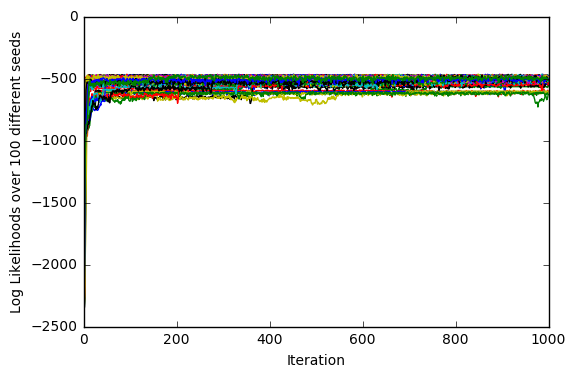
\includegraphics[width = 80mm]{figure1.png}
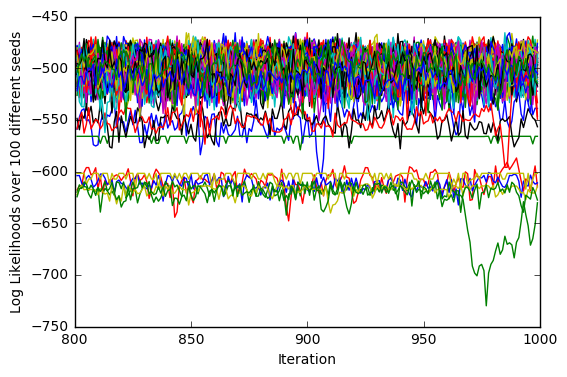
\includegraphics[width = 80mm]{figure2.png}
\caption{The log-likelihoods plot over 100 random seeds.}\scriptsize
\end{figure}
\end{minipage} \\

\noindent The left panel of figure 3 is a plot of loglikelihoods for 2000 interations over seedset2, and the right panel is a closer look at the differences, again there are two clusters. The random seeds used in the higher cluster are [0, 200, 2600, 7800, 13000, 15800](seedset2.1), the random seeds used in the lower cluster are [400, 2800, 3800, 4600, 5800, 12200, 12800, 13000](seedset2.2).\\
\begin{minipage}{1.0\textwidth}
\begin{figure}[H]
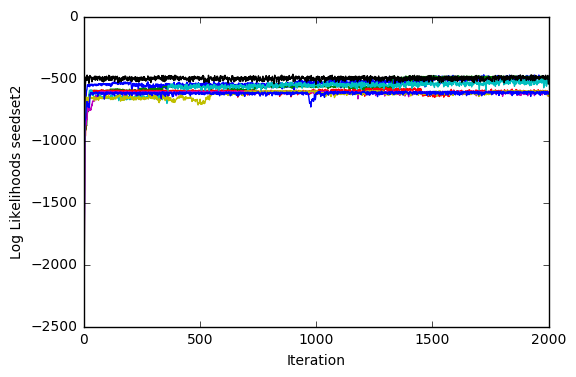
\includegraphics[width = 80mm]{figure3.png}
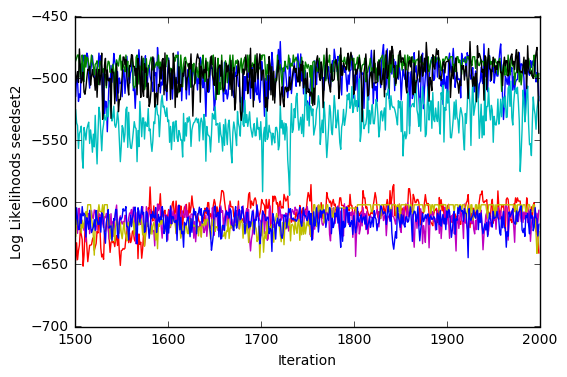
\includegraphics[width = 80mm]{figure4.png}
\caption{The log-likelihoods plot over seedset2.  seedset2= (0, 200, 400, 2600, 2800, 3800, 4600, 5800, 7800, 12200, 12800, 13000, 15800)}\scriptsize
\end{figure}
\end{minipage}\\

\subsection{seedset2.1}
\noindent The left panel of figure 4 is a plot of loglikelihoods over seedset2.1, they all converge to one limit. we can observe that for some seeds in seedset2.1, the loglikelihoods jump from the lower cluster to the higher one (optimal range) at certain iteration. so to examine what happens at those jumps, we listed the values of loglikelihoods and the sampling probabilities topics for each seed in seedset2.1.\\
\begin{minipage}{1.0\textwidth}
\begin{figure}[H]
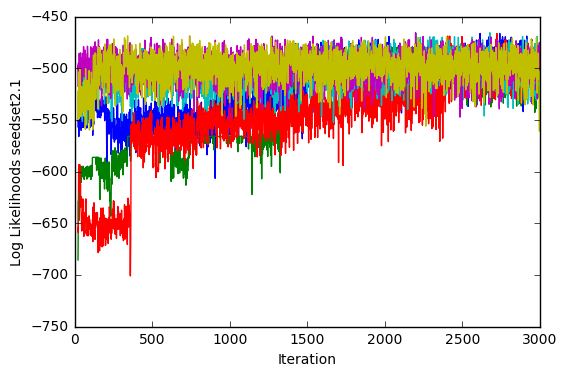
\includegraphics[width = 80mm]{figure5.png}
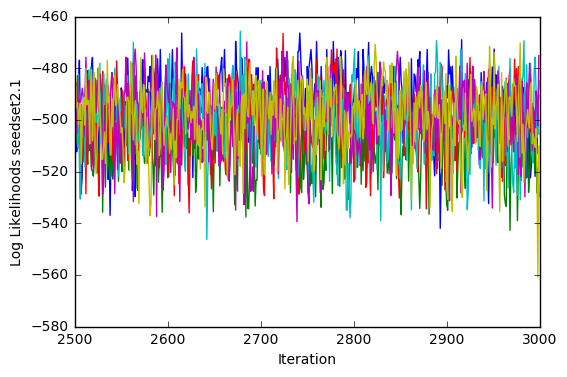
\includegraphics[width = 80mm]{figure6.png}
\caption{The log-likelihoods plot over seedset2.1.  seedset2.1= [0, 200, 2600, 7800, 13000, 15800]}\scriptsize
\end{figure}
\end{minipage}\\





\end{spacing}
\end{document}